\documentclass{article}

\usepackage{notes}
\usepackage{array}
\usepackage{amsmath}
\usepackage{mathtools}
\usepackage{graphicx}
\usepackage{amssymb}
\graphicspath{{./Images/}}

\everymath{\displaystyle}
\DeclarePairedDelimiter{\ceil}{\lceil}{\rceil}

\begin{document}

\title{DMMR Condensed Summary Notes For Quick In-Exam Strategic Fact Deployment }
\author{Maksymilian Mozolewski}
\maketitle
\pagebreak
\nSection{Boolean Logic}
\nDefinition{Equivalence of prepositional statements}{$P \equiv Q$ denotes a logical equivalence between the propositional statements P and Q. Two equivalent propositions have the same truth tables}
\nDefinition{Contrapositive}{let S be a statement of the form $P \rightarrow Q$ then the Contrapositive of S is $\neg Q \rightarrow \neg P$. The Contrapositive of S is logically equivalent to S}
\nTheorem{Boolean Logic Laws}{
\begin{flushleft}
\begin{tabular*}{\textwidth}{lll}
Identity Law: &$P \land T \equiv P$ & $P \lor F \equiv P$\\
Domination Law: &$P \land F \equiv F$ & $P \lor T \equiv T$\\
Idempotency Law: &$P \land P \equiv P$ & $P \lor P \equiv P$\\
Double Negation: &$\neg(\neg P) \equiv P$ &  $ $\\
Commutativity Law: &$P \land Q \equiv Q \land P$ & $P \lor Q \equiv Q \lor P$ \\
Associativity law: &$P \land (Q \land R) \equiv (Q \land P) \land R$ & $P \lor (Q \lor R) \equiv (Q \lor P) \lor R$\\
Distributive Law: &$P \land (Q \lor R) \equiv (P \land Q) \lor (P \land R)$ & $P \lor (Q \land R) \equiv (P \lor Q) \land (P \lor R)$\\
De Morgan's Law: & $\neg(P \land Q) \equiv \neg P \land \neg Q$
\end{tabular*}
\end{flushleft}
}
\nTheorem{Negation of Quantifiers}{
\begin{tabular*}{\textwidth}{ll}
$\neg(\forall x(P(x))) \equiv \exists x \neg P(x)$ & $\neg(\exists x P(x)) \equiv \forall x \neg P(x)$
\end{tabular*}
}
\nSection{Proof Techniques}
\nDefinition{Direct Proof}{use existing propositions and rules of inference to prove the given proposition}
\nDefinition{Proof by Contraposition}{just like direct proof but we use prove contraposition of the given proposition}
\nDefinition{Proof by Contradiction}{let P be the proposition to be proven, then assume $\neg P$ is true and show that $\neg P \rightarrow C$ where C is some logical contradiction of an earlier assumption or fact}
\nSection{Induction}
\nDefinition{Normal Induction}{if P(n) is a predicate on $\mathbb{Z}^{+}$ we follow this process:\\
\emph{Base Case:} we prove P(1) is true\\
\emph{Inductive Hypothesis:} we assume $P(k)$ is true and we set to prove $P(k) \rightarrow P(k + 1)$ is true\\
\emph{Inductive Step:} we show that $P(k) \rightarrow P(k+1)$ is true

}

\nDefinition{Strong Induction}{same as normal induction however instead of assuming P(k) is true, we assume $P(1) \land .. P(k)$ is true and show that it being true implies P(k + 1)}
\nSection{Sets}
\nDefinition{Set}{an unordered collection of objects, called members/elements}
\nDefinition{Important Sets}{
$\mathfbb{B} = \{true,false\}$ Boolean values \\
$\mathfbb{N} = \{0,1,2,3,..\}$ Natural numbers \\
$\mathfbb{Z} = \{...,-3,-2,-1,0,1,2,3,...\}$ Integers \\
$\mathfbb{Z}^{+} = \{z \in \mathfbb{Z} | z > 0\}$ Positive Integers \\
$\mathfbb{R}$ Real Numbers\\ 
$\mathfbb{R}^{+} = \{r\in R | r > 0\}$ Positive Real Numbers \\
$\mathfbb{Q} = \{\frac{a}{b} | a \in \mathbb{Z}, b \in \mathbb{Z}^{+}\}$ Rational Numbers\\
$\mathfbb{Q}^{+} = \{\frac{a}{b} | a \in \mathbb{Z}^{+}, b \in \mathbb{Z}^{+}\}$ Positive Rational Numbers\\
$\mathfbb{C}$ Complex numbers
}
\nDefinition{Power Set}{the power set of a set A consists of all the possible subsets of A including the empty set. if A has n elements, then P(A) will contain $2^{n}$ elements}
\nDefinition{Complement}{the complement of A is the set $\bar{A}$ which contains all the elements which are not in A, relative to the universe of discourse}
\nDefinition{Proofs with sets}{to prove a set is a subset of another, show that an element in the first one must be in the other one, to prove two sets are equal, prove that they are both subsets of each other}
\nTheorem{Set Identities}{
\begin{flushleft}
\begin{tabular*}{\textwidth}{lll}
Identity Law: &$A \cap U = A$ & $A \cup \emptyset = A$\\
Idempotency Law: &$A \cap A = A$ & $A \cup A = A$\\
Commutativity Law: &$A \cap B = B \cap A$ & $A \cup B = B \cup A$\\
De Morgan's Law:&$\overline{A \cap B} = \bar{A} \cap \bar{B}$ & $\overline{A \cup B} = \bar{A} \cup \bar{B}$\\
Absorption Law: &$A \cup (A \cap B) = A$&$A \cap (A \cup B) $\\
Domination Law: &$A \cap \emptyset = \emptyset$&$A \cup U = U$\\
Complementation law: &$ \overline{(\overline{A})} = A$ &$ $\\
Associative Law: &$A \cap (B \cap C) = (A \cap B) \cap C$ & $A \cup (B \cup C) = (A \cup B) \cup C$\\
Distributive Law:& $A \cup (B \cup C) = (A \cup B) \cap (A \cup B)$ &$A \cap (B \cap C) = (A \cap B) \cup (A \cap C)$\\
Complement Law: &$A \cap \overline{A} = \emptyset$&$A \cup \overline{A} = U$\\
\end{tabular*}
\end{flushleft}
}
\nDefinition{Cartesian Product}{$A x B$ is the set of all ordered pairs (a,b) such that $a \in A \land b \in B$}
\nSection{Cardinality}
\nDefinition{Cardinality}{the set A has cardinality $|A|$ which is the number of elements in A}
\nTheorem{Sets comparisons}{for all sets, $|X| \leq |Y|$ iff there is an injection $f: X \rightarrow Y$\\
$|X| = |Y|$ iff there is a bijection $f : X \rightarrow Y$\\
$|X| < |Y|$ iff $|X| \leq |Y| \land |X| \neq |Y|$}
\nDefinition{Countability}{A set S is called countably infinite, iff it has the same cardinality as the positive integers, $|\mathbb{Z}^{+}| = |S|$ we then say it has cardinality $\aleph$\\ A set is called countable iff it is either finite or countably infinite, otherwise it's called uncountable}
\nTheorem{Countability and Union}{if A and B are countable sets, then $A\cup B$ is countable}
\nTheorem{Countability of Big Union}{if I is countable and for each $i \in I$ the set $A_{i}$ is countable then $\bigcup_{i\in I} A_{i}$ is countable}
\nTheorem{Cardinality of Finite Strings}{The set $\sum^{*}$ of all finite strings over a finite alphabet $\sum$ is countably infinite}
\nTheorem{Uncountable sets}{The set of infinite binary strings is uncountable\\The set $[0,1] \subseteq R$ is uncountable\\The set of functions $F = \{f|f : \mathbb{Z} \rightarrow \mathbb{Z}\}$ is uncountable}
\nTheorem{Schroder-Bernstein Theorem}{if $|A| \leq |B| \land |B| \leq |A|$ then $|A| = |B|$}
\nTheorem{Cantor's theorem}{$|A| < |P(A)|$}
\nTheorem{Continuum}{the cardinality of the set $\mathbb{R}$ is $\mathfrak{c}$, and $\aleph < \mathfrak{c}$, there exists an infinite hierarchy of cardinalities of infinite sets}
\nSection{Relations}
\nDefinition{Binary relation}{a binary relation R on sets A and B is a subset $R \subseteq A x B$. e.g. a set of tuples (a,b) with $a \in A \land b \in B$}
\nDefinition{n-ary relation}{given sets $A_{1},...,A_{n}$ a subset $R \subseteq A_{1},...,A_{n}$ is an n-ary relation}
\nTheorem{Relation Union and Intersection}{if $R_{i}$ are relations on $AxB \forall i \in I$ then $\bigcup_{i\in I}R_{i}$ and $\bigcap_{i\in I}R_{i}$ are relations on AxB}
\nDefinition{Relation composition}{let $R \subseteq BxC$ and $S \subseteq A x B$ the composition relation $(R \circ S) \subseteq A x C$ is\\ $\{(a,c) | \exists b(a,b) \in S \land (b,c) \in R\}$}
\nDefinition{Closures}{Closure R is a relation on A: 
\begin{itemize}
    \item $R^{0}$ is the identity relation $(\mathbf{i}_{A})$
    \item $R^{n+1} = R^{n} \circ R$
    \item $R^{*} = \bigcup_{n \geq 0} R^{n}$
\end{itemize}
$R^{*}$ is the reflexive and transitive closure of R}
\nDefinition{Properties of binary relations}{the relation R on A is:\\
reflexive iff $\forall x \in A. (x,x) \in R$\\
symmetric iff $\forall x,y \in A. ((x,y) \in R \rightarrow (y,x) \in R)$\\
antisymmetric iff $\forall x,y \in A (((x,y) \in R \land (y,x) \in R) \rightarrow x = y)$\\
transitive iff $\forall x,y,z \in A(((x,y)\in R \land (y,z) \in R) \rightarrow (x,z) \in R)$}
\nDefinition{Equivalence relations}{A relation R on a set A is an equivalence relation iff it is reflexive, symmetric and transitive}
\nDefinition{Equivalence classes}{let R be an equivalence relation on a set A and $a\in A$. Then\\ $[a]_{R} = \{s|(a,s \in R)\}$\\
is the equivalence class of a w.r.t R}
\nTheorem{Properties on equivalent relations}{let R be an equivalence relation on A and a,b $\in A$ the following three statements are equivalent:
\begin{itemize}
    \item aRb
    \item $[a]_{R} = [b]){r}$
    \item $[a]_{R} \cap [b]){r} \neq \emptyset$
\end{itemize}
}
\nDefinition{Partitions of a set}{A partition of a set A is a collection of disjoint, nonempty subsets that have A as their union.}
\nTheorem{Equivalence To Partition}{If R is an equivalence on A, then the equivalence classes of R form a partition of A. Conversely, given a partition ${A_{i}|i \in I}$ of A there exists an equivalence relation R that has exactly the sets $A_{i}$ for $i \in I$ as its equivalence classes}
\nSection{Functions}
\nDefinition{Function}{let A and B be a non-empty set, then a function f maps exactly one element of B to each element of A. so every element in the function must be defined on all elements in A and there cannot be more than one element of B associated with any element of A}
\nDefinition{function Composition}{if f and g are functions then $f \circ g = f(g(x))$}
\nTheorem{new Functions from old functions}{if f and g are functions then $f + g$ and $f \circ g$ is also a function\\
if f and g are both injective/surjective/bijective then $f\circ g$ is also injective/surjective/bijective (respectively)}
\nDefinition{Injective Functions (one-to-one)}{$f: A\rightarrow B$ is injective iff $\forall a,c \in A (f(a) = f(c) \rightarrow a = c)$}
\nDefinition{Surjective Functions (onto)}{$f : A \rightarrow B$ is surjective iff $\forall b\in B\exists a\in A(f(a) = b)$}
\nDefinition{Bijective Functions (One-to-one correspondence)}{$f : A \rightarrow B$ is a bijection iff it is both injective and surjective}

\nDefinition{Inverse Functions}{let $f : A \rightarrow B$ be a bijection, then the inverse of f, $f^{-1}: B \rightarrow A$ is $f^{-1}(b) = a$ iff $f(a) = b$. So the inverse function exists only for bijections, and it exists for only the elements in B which are mapped to by some element $a \in A$ by f}
\nSection{Sequences}
\nDefinition{Sequences}{Sequences are ordered lists of elements, \\
Example: $f : \mathbb{Z}^{+} \rightarrow \mathbb{Q} f(n) = \frac{1}{n}$ defines the sequence $1,1/2,1/3,1/4,...$ assuming $a_{n} = f(n)$ the sequence is also written $a_{1},a_{2},a_{3}...$ or as $\{a_{n\in\mathbb{Z}^{+}}\}$}
\nDefinition{Sequence over a Set}{a sequence over a set S is a function f from a subset of the integers to the set S. If the domain of f is finite then the sequence is finite.}
\nDefinition{Geometric and Arithmetic progressions}{A geometric progression is a sequence of the form $a, ar, ar^{2},...ar^{n},..$\\
An arithmetic progression is a sequence of the form $a, a + d, a + 2d,...,a + nd$, where the initial elements a, the common ratio r and the common difference d are real numbers}
\nDefinition{Reccurence relations}{A reccurencerelation for $\{a_{n}\}_{n\in \mathbb{N}}$ is an equation that expresses $a_{n}$ in terms of one or more of the elements $a_{0},a_{1},...,a_{n-1}$\\
the initial conditions specify the first elements of the sequence, before the recurrence relation applies\\
A sequence is called a solution of a recurrence relation iff its terms satisfy the recurrence relation}
\nDefinition{Fibonnaci Sequence}{
    \begin{equation*}
        f(x) = 
        \begin{cases}
            1 & n = 1\\
            1 & n = 2\\
            f(n-1) + f(n-2) & n > 2\\
       \end{cases}
    \end{equation*}
    }
\nDefinition{Solving recurrence relations with iteration}{$a_{n} = a_{n-1} + 3$ for $n \geq 2$ with $a_{1} = 2$\\ Forward Substitution Method:\\
$a_{2} = 2 + 3$\\
$a_{3} = (2 + 3) + 3 = 2 + 3 \cdot 2$\\
$a_{4} = (2 + 2 \cdot 3) + 3 = 2 + 3 \cdot 3$\\
& \vdots \notag \\
$a_{n} = a_{n-1} + 3 = (2 + 3 \cdot (2 - 2)) + 3 = 2 + 3 \cdot (n-1)$\\
Backward Substitution Method:\\
$a_{n} = a_{n-1} + 3$\\
$\hspace{7}= a_{n-2} + 3 = a_{n-2} + 3 \cdot 2$\\
$\hspace{7}= a_{n-3} + 3 \cdot 2 = a_{n-2} + 3 \cdot 3$\\
& \vdots \notag \\
$\hspace{7}= a_{2} + 3(n - 2) = (a_{1} + 3) + 3 \cdot (n-2) = 2 + 3(n-1)$\\
}
\nDefinition{Common Sequences}{
\begin{tabular*}{0.7\textwidth}{l|l}
    nth Term & First 10 terms\\
    \hline
    $n^{2}$ & $1,4,9,16,25,36,49,64,81,100,...$\\
    $n^{3}$ & $1,8,27,64,125,216,343,512,729,1000,...$\\
    $n^{4}$ & $1, 16, 81, 256, 625, 1296, 2401, 4096, 6561, 10000,...$\\
    $2^{n}$ & $ 2, 4, 8, 16, 32, 64, 128, 256, 512, 1024,...$\\
    $3^{n}$ & $ 3, 9, 27, 81, 243, 729, 2187, 6561, 19683, 59049,...$\\
    $n!$ & $ 1, 2, 6, 24, 120, 720, 5040, 40320, 362880, 3628800,...$\\
    $f_{n}$ & $ 1, 1, 2, 3, 5, 8, 13, 21, 34, 55, 89,...$\\ 
    \end{tabular*}
}
\nSection{Sums}
\nDefinition{Sums}{
given a sequence $\{a_{n}\}$, the sum of terms $a_{m},a_{m+1},...,a_{\mathfbb{l}}$ is \\
\begin{gather*}
    a_{m} + a_{m+1} + ... + a_{\mathfbb{l}} \text{ or}\\
    \sum_{j=m}^{\mathbb{l}}{a_{j}} \text{ or } \sum_{m\leq j \leq \mathfbb{l}}{a_{j}} 
\end{gather*}
more generally for an index set S: 
\begin{equation*}
    \sum_{j\in S}{a_{j}}
\end{equation*}
}
\nTheorem{Useful Summation Formulas}{
\begin{tabular*}{0.45\linewidth}{l|l}
Sum & Closed Form\\
\hline\\[1pt]
 $\sum_{k=0}^{n}{ar^{k}} (r \neq 0)$ & $\frac{ar^{n+1}-a}{r-1} , r\neq 1$\\[15pt]
$\sum_{k=1}^{n}{k}$ & $\frac{n(n+1)}{2}$\\[15pt]
$\sum_{k=1}^{n}{k^{2}}$ & $\frac{n(n+1)(2n+1)}{6}$\\[15pt]
$\sum_{k=1}^{n}{k^{3}}$ & $\frac{n^{2}(n+1)^{2}}{4}$\\[15pt]
$\sum_{k=0}^{\infty}{x^{k}, |x| < 1}$ & $\frac{1}{1-x}$\\[15pt]
$\sum_{k=1}^{\infty}{kx^{k-1}, |x| < 1}$ & $\frac{1}{(1-x)^{2}}$
\end{tabular*}
}
\nDefinition{Products}{
given a sequence $\{a_{n}\}$, the product of terms $a_{m},a_{m+1},...,a_{\mathfbb{l}}$ is \\
\begin{gather*}
    a_{m} + a_{m+1} + ... + a_{\mathfbb{l}} \text{ or}\\
    \prod_{j=m}^{\mathbb{l}}{a_{j}} \text{ or } \prod_{m\leq j \leq \mathfbb{l}}{a_{j}} 
\end{gather*}
more generally for an index set S: 
\begin{equation*}
    \prod_{j\in S}{a_{j}}
\end{equation*}
}
\nSection{Number Theory}
\nDefinition{Division}{if a and b are integers with $a \neq 0$, then a divides b, written $a|b$, if there exists an integer c such that $b = ac$}
\nTheorem{Divisibility Results}{
if $a,b,c$ are integers, then the following hold:
\begin{itemize}
    \item $a|b \land a|c \rightarrow a|(b+c) \land a|(b-c)$
    \item $a|b \rightarrow a|bc$
    \item $a|b \land b|c \rightarrow a|c$
\end{itemize}
}
\nTheorem{Division Algorithm}{if a is an integer and d is a positive integer, then there are unique integers q and r, with $0 \leq r < d$, such that $a = dq + r$.\\ q is the quotient, r is the remainder, q = a div b and r = a mod d}
\nDefinition{Congruency}{
if a and b are integers and m is a positive integer, then\\ a is congruent to b modulo m, written $a \equiv b$ (mod m), iff $m|(a-b)$}
\nTheorem{Congruence is an equivalence relation}{$a \equiv b$ (mod m) iff a mod m = b mod m}
\nTheorem{Congruence Result}{$a\equiv b$ (mod m) iff there is an integer k such that a = b + km}
\nTheorem{Congruences of sums,differences and products}{
if $a\equiv b$ (mod m) and $c \equiv d$ (mod m), then $a + c \equiv b + d$ (mod m) and $ac \equiv bd$ (mod m)}
\nTheorem{Corollary}{
\begin{itemize}
    \item $(a + b)$ (mod m) = ((a mod m) + (b mod m)) mod m
    \item $ab$ mod m = ((a mod m)(b mod m)) mod m
\end{itemize}}
\nDefinition{Arithmetic modulo m}{$\mathbb{Z}_{m} = \{0,1,...,m-1\}$\\
$+_{m}$ on $\mathbb{Z}_{m}$ is $a +_{m}b = (a + b)$ mod m\\
$\cdot_{m}$ on $\mathbb{Z}_{m}$ is $a \cdot_{m}b = (a + b)$ mod m}
\nDefinition{Primes}{A positive integer p > 1 is called \emph{prime} iff the only positive factors of p are 1 and p. otherwise it is called \emph{composite}}
\nTheorem{Fundamental Theorem of Arithmetic}{Every positive integer greater than 1 can be written uniquely as a prime or as the product of its prime factors, written in order of non-decreasing size}
\nTheorem{Lemma}{ if p is prime and $p|a_{1}a_{2}...a_{n}$ where each $a_{i}$ is an integer, then $p|a_{j}$ for some $1 \leq j \leq n $}
\nTheorem{Infinity of primes}{Every natural number greater than one is either prime or it has a prime divisor and there are infinitely many primes}
\nTheorem{Trial Division}{if n is a composite integer, then n has a prime divisor less than or equal to $\sqrt{n}$}
\nDefinition{The Sieve of Eratosthenes}{To find all primes between 2 and n:\\
try every integer $i \leq \sqrt{n}$ and see if n is divisible by i
\begin{itemize}
    \item write the numbers 2,..,n into a list. Let i := 2
    \item remove all strict multiples of i from the list
    \item let k be the smallest number present in the list s.t k > i and let i:= k
    \item if $i > \sqrt{n}$ then stop else go to step 2
\end{itemize}
}
\nDefinition{Greatest Common Divisor}{
Let a, b ∈ Z
+.The largest integer d such that $d|a$ and $d|b$ is called the
greatest common divisor of a and b, written gcd(a, b)}
\nDefinition{Coprimes}{The integers a and b are relatively prime (coprime) iff gcd(a, b) = 1}
\nTheorem{GCD from prime factors}{gcd(a,b) = $p_{1}^{min(a_{1},b_{1})}p_{2}^{min({a_{1},b_{2})}}...p_{n}^{min({a_{n},b_{n})}}$}
\nTheorem{Euclidian Algorithm}{if x and y are integers and $x \geq y$ then\\ gcd(x,y) = gcd(y,x mod y) and\\
gcd(x,0) = x}
\nTheorem{Bezout's Theorem}{If x and y are positive integers,then \\there exist integers a and b such
that gcd(x, y) = ax + by}
\nTheorem{Extended Euclidian algorithm}{
algorithm e-gcd(x,y)\\
\hspace*{6mm} if y = 0\\
\hspace*{6mm} then return(x, 1, 0)\\
\hspace*{6mm} else\\
\hspace*{10mm} (d, a, b) := e-gcd(y, x mod y)\\
\hspace*{10mm} return((d, b, a - ((x div y) * b)))\\
\emph{example:}\\
e-gcd(22,4) = (2,1,0-($5\cdot 1$)) = (2,1,-5)\\
e-gcd(4,2) = (2,0,1-($2 \cdot 0$)) = (2,0,1)\\
e-gcd(2,0) = (2,1,0)\\
so gcd(22,4)$ = 2 = 1 \cdot 22 + (-5) \cdot 4$
}
\nTheorem{Properties}{if a,b,c are positive integers such that gcd(a,b) = 1 and $a|bc$ then $a|c$\\ i.e. if a has no common factors with b (except 1) but has common factors with bc then a has common factors with c}
\nTheorem{Further Properties}{let m be a positive integer and let a,b,c be integers.\\ if $ac \equiv bc$ (mod m) and gcd(c,m) = 1, then $a \equiv b$ (mod m)}
\nDefinition{Multiplicative Inverses}{let x,y,m be integers, then y is a multiplicative inverse modulo m of x when $xy \equiv 1$ (mod m)}
\nTheorem{Existence of inverses}{if m,x are positive integers and gcd(m,x) = 1 then x has a multiplicative inverse mod m (and it is unique mod m)}

\nTheorem{Chineese Reminder Theorem}{
Let $m_{1},...,m_{n}$ be pairwise relatively prime positive integers greater than 1 and $a_{1},...,a_{n}$ be arbitrary integers. Then the system:
\begin{gather*}
    x \equiv a_{1} \Mod{m_{1}}\\
    x \equiv a_{2} \Mod{m_{2}}\\
    \vdots\\
    x \equiv a_{n} \Mod{m_{n}}
\end{gather*}
has a unique solution modulo $m = m_{1}m_{2}\cdots m_{n}$\\
here is a general construction to find such solution:\\
\begin{itemize}
    \item Compute M = $m_{1}m_{2}\cdots m_{n}$
    \item for each i = 1,2,...,n, compute: $y_{i} = \frac{M}{m_{i}} = m_{1}m_{2}\cdots m_{i-1}m_{i+1}\cdots m_{n}$
    \item for each i = 1,2,...,n, compute $z_{i} \equiv y_{i}^{-1} \Mod{m_{i}}$ (the inverse of each y, can be found using the e-gcd algorithm by taking the result of $e-gcd(m_{i},y_{i})$ = ($1 = a\cdot y_{i} + b\cdot m_{i})$ and taking $\Mod{m_{i}}$ of both sides)
    \item the integer $x = \sum_{i=1}^{k}{a_{i}y_{i}z_{i}}$ is a solution to the system of congruences and x mod N is the unique solution modulo M
\end{itemize}
any other solutions will be multiples of M
}
\nTheorem{Fermat's little Theorem}{if p is prime and $p \not| \;a$ then $a^{p-1} \equiv 1 \Mod{p}$. Furthermore, for every integer a we have:\\ $a^{p}\equiv a\Mod{p}$}
\nDefinition{RSA cryptography}{Choose two distinct prime numbers pand q\\
let n = pq and k = (p-1)(q-1)\\
choose integer e where 1 < e < k and gcd (e,k) = 1\\
(n,e) is released as the public key\\
let d be the multiplicative inverse of e modulo k, so $de \equiv 1 \Mod k$\\
(n,d) is the private key and kept secret\\
Encryption:
\begin{itemize}
    \item Bob has public key (n,e) but no private key
    \item turns M into integer m, $0 \leq m < n$, using an agreed-upon reversible protocol - the padding scheme
    \item he computes the ciphertext c corresponding to $c = m^{e}$ mod n.
    \item Bob transmits c to alice
\end{itemize}
Decryption:
\begin{itemize}
    \item using her private key (n,d), computes $m = c^{d}$ mod n
    \item given m, she can recover the original message M by reversing the padding scheme
\end{itemize}
}
\nSection{Counting}
\nTheorem{Product Rule}{if A and B are finite sets then: $|A x B| = |A| \cdot |B|$}
\nTheorem{General Product Rule}{if $A_{1},A_{2},...,A_{m}$ are finite sets then: $|A_{1},A_{2},...,A_{m}| = |A_{1}|\cdot|A_{2}|\cdots|A_{m}|$}
\nTheorem{Counting Subsets}{A finite set, S, has $2^{|S|}$ distinct subsets}
\nTheorem{Counting Functions}{For all finite sets A and B, the number of distinct functions, $f : A \rightarrow B$, mapping A to B is:
\begin{align*}
    |B|^{|A|}
\end{align*}
}
\nTheorem{Sum Rule}{if A and B are finite sets that are disjoint, then:
\begin{align*}
    |A\cup B| = |A| + |B|
\end{align*}}
\nTheorem{General Sum Rule}{
if $A_{1},...,A_{m}$ are finite sets that are pairwise disjoint, then:
\begin{align*}
    |A_{1},...,A_{m}| = |A_{1}| +...+ |A_{m}| 
\end{align*}}
\nTheorem{Pigeonhole Principle}{For any positive integer k, if k + 1 objects (pigeons) are placed in k
boxes (pigeonholes), then at least one box contains two or more
objects.}
\nTheorem{Generalized Pigeonhole Principle}{If N ≥ 0 objects are placed in k ≥ 1 boxes, then at least one box contains at least $\ceil[\bigg]{\frac{N}{k}
}$
objects}
\nDefinition{Permutations}{A permutation of a set S is an ordered arrangement of the elements
of S.
In other words, it is a sequence containing every element of S exactly
once}
\nDefinition{R-Permutations}{An r-permutation of a set S, is an ordered arrangement (sequence) of
r distinct elements of S.
(For this to be well-defined, r needs to be an integer with $0 \leq r \leq |S|.)$}
\nTheorem{Calculating r-permutations}{let P(n,r) denote the number of r-permutations of an n-elements set. For all integers $n \geq 1$, and all integers r such that $1 \leq r \leq n$: \\P(n,r) = $\frac{n!}{(n-r)!}$}
\nTheorem{How big is n!}{$n! \leq n^{n}$ for all n bigger than 0\\
$2^{n} < n!$ for all n bigger or equal than 4}
\nTheorem{Stirling's approximation formula}{
$n! \approx \sqrt{2\pin} \cdot (\frac{n}{e})^{n}$ or \\
\begin{align*}
    \sqrt{2\pin} \cdot (\frac{n}{e})^{n} \cdot e^{\frac{1}{12n + 1}} \leq n! \leq \sqrt{2\pin} \cdot (\frac{n}{e})^{n} \cdot e^{\frac{1}{12n}}
\end{align*}}
\nDefinition{R-Combinations}{An r-combination of a set S is an unordered collection of r elements
of S. In other words, it is simply a subset of S of size r}
\nTheorem{Calculating R-Combinations}{
let C(n,r) denote the number of r-combinations of an n-element set, which is also written as $n\choose r$. Then for all integers $n \geq 1$, and for all integers r such taht $0 \leq r \leq n$:\\
\begin{align*}
    C(n,r) = {n \choose r} = \frac{n!}{r! \cdot (n-r)!} = \frac{n\cdot(n-1)\cdots(n-r+1)}{r!}
\end{align*}}
\nTheorem{Bounds for Combinations}{
using basic considerations and stirling's approximation formula, one can easilly estabilish the following bounds and approximations for $n \choose r$:
\begin{gather*}
    (\frac{n}{r})^{r} \leq {n \choose r} \leq (\frac{n\cdot e}{r})^{r}\\
    {2n \choose n} \approx \frac{2^{2n}}{\sqrt{\pi n}}\\
    \frac{2^{2n}}{2n+1} \leq {2n \choose n} \leq 2^{2n}
\end{gather*}}
\nTheorem{Combinations Identity}{For all integers $n \geq 1$ and all integers r $1 \leq r \leq n$:\\
\begin{align*}
    {n \choose r} = {n \choose n-r}
\end{align*}}
\nTheorem{The Binomial Theorem}{For all $n \geq 0$:
\begin{align*}
    (x + y)^{n} = \sum_{j=0}^{n}{{n \choose j}x^{n-j}y^{j}}
\end{align*}
}
\nTheorem{Corollary}{
\begin{align*}
    \sum_{j=0}^{n}{n\choose j} = 2^{n}
\end{align*}}
\nTheorem{Pascal's Identity}{
For all integers $n \geq 0$, and all integers r, $0 \leq r \leq n+1$:
\begin{align*}
    {n+1 \choose r} = {n\choose r-1} + {n \choose r}
\end{align*}
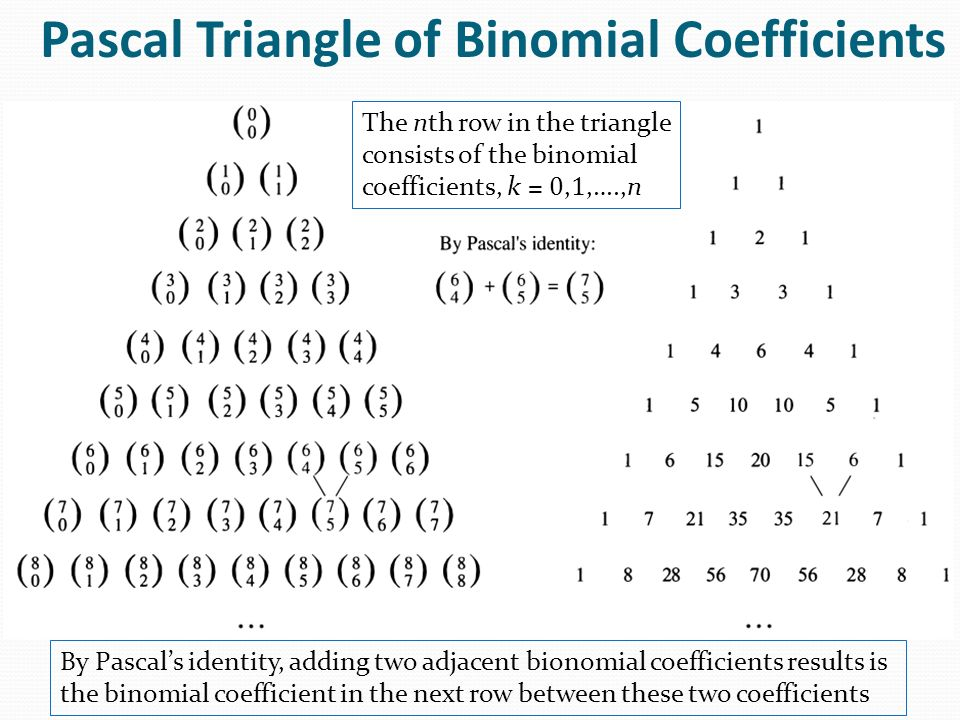
\includegraphics[scale=0.55]{Triangle}}
\nTheorem{Vandermonde's identity}{
for m,n,r $\geq 0$, r $\leq m$ and r $\leq$ n, we have:
\begin{align*}
    {m + n \choose r} = \sum_{k=0}^{r}{m \choose r-k}{n \choose k}
\end{align*}}
\nDefinition{R-Combinations with repetition}{from a set S is simply a multi-set of size r over S (set which can contain multiple of each element)}
\nTheorem{counting r-combinations with repetition}{
For all integers n,r $\geq 1$, the number of r-combs-w.r. from a set S of size n is
\begin{align*}
    {n+r-1\choose r} = {n+r-1 \choose n-1}
\end{align*}}
\nTheorem{}{The number of permutations of n objects, with $n_{1}$
indistinguishable objects of Type 1, $n_{2}$ indistinguishable objects of Type
2,..., and $n_{k}$ indistinuishable objects of Type k, is: 
\begin{align*}
    {n \choose n_{1},n_{2},...,n_{k}} = \frac{n!}{n_{1}!n_{2}!...n_{k}!}
\end{align*}}
\nTheorem{Multinomial theorem}{for all n $\geq$ 0 and all k $\geq 1$:
\begin{align*}
    ({x_{1}+x_{2}+...+x_{k}})^{n} = \sum_{0\leq n_{1},n_{2},...,n_{k}\leq n}{n\choose n_{1},n_{2},...,n_{k}}x_{1}^{n_{1}}x_{2}^{n_{2}}...x_{k}^{n_{k}}
\end{align*}}
\nSection{Graphs}
\nDefinition{Graph Types}{
\begin{tabular*}{\textwidth}{l|l|l|l}
     \emph{Type} & \emph{Edges} & \emph{Multi-Edges} & \emph{Loops}\\
     \hline
     (simple undirected) graph & Undirected & No & No \\
     (undirected) multigraph & Undirected & Yes & No \\
     (undirected) pseudograph & Undirected & Yes & Yes\\
     directed graph & Directed & No & Yes\\
     simple directed graph & Directed & No & No \\
     directed multigraph & Directed &Yes& No\\
     directed pseudograph & Directed &Yes & Yes\\
     mixed graph & Both & Yes& Yes
\end{tabular*}
}
\nDefinition{Directed Graph Definition}{A directed graph (digraph), G = (V, E), consists of a non-empty set,
V, of vertices (or nodes), and a set $E \subseteq V × V$ of directed edges (or
arcs). Each directed edge $(u, v) \in E$ has a start (tail) vertex u, and a
end (head) vertex v.
Note: a directed graph G = (V, E) is simply a set V together with a
binary relation E on V}
\nDefinition{Undirected Graph Definition}{
A (simple,undirected) graph, G = (V, E), consists of a non-empty set
V of vertices (or nodes), and a set$ E \subseteq [V]$
2
of (undirected) edges.
Every edge ${u, v} \in E$ has two distinct vertices u 6= v as endpoints,
and such vertices u and v are then said to be adjacent in the graph G.}
\nDefinition{Degree of a vertex}{
The degree of a vertex v in a
undirected graph is the number of edges
incident with it. The degree of the vertex v is
denoted by deg(v).}
\nDefinition{The Neighbourhood of a vertex}{
The neighborhood (neighbor set)
of a vertex v in a undirected graph, denoted
N(v) is the set of vertices adjacent to v.}
\nTheorem{Handshaking Theorem}{
 If
G=(V,E) is a undirected graph with m edges. let $V_{1}$ be the vertices of even degree and $V_{2}$ be the vertices of odd degree in G,
then:
\begin{align*}
    2m = \sum_{v \in V}deg(v) = \sum_{v \in V_{1}}deg(v) + \sum_{v \in V_{2}}deg(v)
\end{align*}}
\nDefinition{In/Out degree}{
The in-degree of a vertex v,
denoted $deg_{-}(v)$, is the number of edges
directed into v. The out-degree of v, denoted
$deg_{+}(v)$, is the number of edges directed out of
v. Note that a loop at a vertex contributes 1 to
both in-degree and out-degree.}
\nTheorem{Number of Edges of a Directed Graph}{
 Let G = (V, E) be a directed graph.
Then:
\begin{align*}
    |E| = \sum_{v \in V}deg^{-}(v) = \sum_{v \in V}deg^{+}(v)
\end{align*}}
\nDefinition{Complete Graphs}{
A \emph{complete graph} on n vertices, denoted by $K_{n}$
is the simple graph that contains exactly one
edge between each pair of distinct vertices.}
\nDefinition{Cyclical Graphs}{
A cycle $C_{n}$ for $n \geq 3$ consists of n vertices $v_{1},v_{2},v_{n}$ and edges \\ $(v_{1},v_{2}),(v_{2},v_{3}),...,(v_{n-1},v_{n}),(v_{n},v_{1})$
}
\nDefinition{n-Cubes}{
An n-dimensional hypercube, or n-cube, is a
graph with $2^{n}$ vertices representing all bit
strings of length n, where there is an edge
between two vertices if and only if they differ in
exactly one bit position.}
\nDefinition{Bipartite Graphs}{
An equivalent definition of a bipartite graph is
one where it is possible to color the vertices
either red or blue so that no two adjacent
vertices are the same color.}
\nDefinition{Complete Bipartite Graphs}{
A complete bipartite graph
is a graph that has its vertex set partitioned
into two subsets $V_{1}$ of size m and $V_{2}$ of size n
such that there is an edge from every vertex in
$V_{1}$ to every vertex in $V_{2}$.}
\nDefinition{Subgraphs}{
A subgraph of a graph G =
(V,E) is a graph (W,F), where
$W \subseteq V$ and $F \subseteq E$. A subgraph H of G is a proper
subgraph of G if $H \neq G$.}
\nDefinition{Induced Subgraphs}{
Let G = (V, E) be a graph. The
subgraph induced by a subset W of the vertex
set V is the graph H= (W,F), whose edge
set F contains an edge in E if and only if both
endpoints are in W. }
\nDefinition{Bipartite Graph alternative Definition}{
A bipartite graph is a (undirected) graph G = (V,E) whose
vertices can be partitioned into two disjoint sets $(V_{1},V_{2}
)$, with
$V_{1} \cap V_{2} = \emptyset$ and $V_{1} \cup V_{2} = V$, such that for every edge $e \in E$,
e = \{u, v\} such that $u \in V_{1}$
and $v \in V_{2}$. In other words, every
edge connects a vertex in $V_{1}$ with a vertex in $V_{2}$.\\
Equivalently, a graph is bipartite if and only if it is possible to
color each vertex red or blue such that no two adjacent vertices
are the same color.
}
\nDefinition{Matchings}{
A \textbf{matching}, M, in a graph, G = (V,E), is a subset of edges,
$M \subseteq E$, such that there does not exist two distinct edges in M
that are incident on the same vertex. In other words, if
$\{u, v\}, \{w, z\} \in M$, then either $\{u, v\} = \{w, z\}$ or
$\{u, v\} \cap \{w, z\} = \emptyset.$\\\\
A \textbf{maximum matching} in graph G is a matching in G with the
maximum possible number of edges.}
\nDefinition{Perfect/Complete Matchings}{
For a graph G = (V,E), we say that a subset of edges, $W \subseteq E$,
\textbf{covers} a subset of vertices, $A \subseteq V$, if for all vertices $u \in A$,
there exists an edge $e \in W$, such that e is incident on u, i.e.,
such that e = \{u, v\}, for some vertex v.\\\\
In a bipartite graph G = (V,E) with bipartition $(V_{1},V_{2}
)$, a
\textbf{complete matching} with respect to $V_{1}$, is a matching $M^{'}
\subseteq E$
that covers $V_{1}$, and a \textbf{perfect matching} is a matching, $M_{*}
\subseteq E$,
that covers V.
}
\nTheorem{Hall's Marriage Theorem}{
For a bipartite graph G = (V,E), with bipartition $(V_{1},V_{2}
)$, there
exists a matching $M \subseteq E$ that covers $V_{1}$ if and only if for all
$S \subseteq V_{1}, |S| \leq |N(S)|$.}
\nTheorem{Corollary}{
Corollary A bipartite graph G = (V,E) with bipartition $(V_{1},V_{2}
)$
has a perfect matching if and only if $|V_{1}| = |V_{2}|$ and $\forall S \subseteq V_{1},
|S| \leq |N_{G}(S)|$.}
\nTheorem{New Graphs From Old}{
The union of two simple graphs
 $G_{1} = (V_{1}, E_{1})$ and $G_{2} = (V_{2}, E_{2})$ is the
simple graph with vertex set $V_{1} \cup V_{2}$ and edge
set $E_{1} \cup E_{2}$. The union of $G_{1}$ and $G_{2}$ is denoted
by $G_{1} \cup G_{2}$.}
\nDefinition{Representing Graphs: Adjacency Lists}{
 An \textbf{adjacency list} represents a
graph (with no multiple edges) by specifying
the vertices that are adjacent to each vertex.
}
\nDefinition{Adjacency Matrix}{
Suppose that G = (V, E) is a simple
graph where $|V| = n$. Arbitrarily list the vertices
of G as $v_{1}, v_{2},..., v_{n}.$
The adjacency matrix, A, of G, with respect to
this listing of vertices, is the $n \: x \: n$ 0-1 matrix
with its (i, j)th entry = 1 when $v_{i}$ and $v_{j}$ are
adjacent, and = 0 when they are not adjacent}
\nDefinition{Isomorphism of graphs}{
Definition: Two (undirected) graphs
$G_{1} = (V_{1}, E_{1})$ and $G_{2} = (V_{2}, E_{2})$ are
isomorphic if there is a bijection, ,
with the property that for all vertices $a,b \in V_{1}$
\begin{align*}
    \{a,b\}\in E_{1} \; \text{if and only if} \; \{f(a),f(b)\}\in E_{2}
\end{align*}
Such a function f is called an isomorphism.
Intuitively, isomorphic graphs are “THE SAME”,
except for “renamed” vertices.}
\nDefinition{Paths}{
For an undirected graph(same definition for directed graphs) G = (V,E), an integer
$n \geq 0$, and vertices $u, v \in V,$ \textbf{a path (or walk) of length n from u
to v} in G is a sequence:\\
$x_{0}, e_{1}, x_{1}, e_{2},..., x_{n−1}, e_{n}, x_{n}$\\
of interleaved vertices $x_{j} \in V$ and edges $e_{i} \in E$,
such that $x_{0} = u$ and $x_{n} = v$, and such that $e_{i} = \{x_{i−1}, x_{i}
\} \in E$ for
all $i \in {1,..., n}.$\\
Such a path \textbf{starts} at u and \textbf{ends} at v. A path of length $n \geq 1$ is
called a \textbf{circuit (or cycle)} if $n \geq 1$ and the path starts and ends at
the same vertex, i.e., u = v.\\
A path or circuit is called \textbf{simple} if it does not contain the same
edge more than once.(And we call it \textbf{tidy} if it does not contain the same vertex more than once, except possibly the first and last in case u = v and the path is a circuit (cycle))
}
\nDefinition{Connectedness in Undirected Graphs}{
An undirected graph G = (V,E) is called connected,
if there is a path between every pair of distinct vertices.
It is called disconnnected otherwise.\\ \\ There is always a simple, and tidy path between any pair of vertices u,v of a connected undirected graph G.
}
\nDefinition{Connected Components}{
A connected component $H = (V^{'},E^{'})$ of a graph
G = (V,E) is a maximal connected subgraph of G, meaning H
is connected and $V^{'}
\subseteq V$ and $E^{'}
\subseteq E$, but H is not a proper
subgraph of a larger connected subgraph R of G.
}
\nDefinition{Connectedness in Directed Graphs}{
A directed graph G = (V,E) is called \textbf{strongly
connected}, if for every pair of vertices u and v in V, there is a (directed) path from u to v, and a directed path from v to u.\\\\
(G = (V,E) is \textbf{weakly connected} if there is a path between
every pair of vertices in V in the underlying undirected graph
(meaning when we ignore the direction of edges in E.)\\\\
A \textbf{strongly connected component (SCC)} of a directed graph G,
is a maximal strongly connected subgraph H of G which is not
contained in a larger strongly connected subgraph of G
}
\nDefinition{Directed Acyclic Graph (DAG)}{
A Directed Acyclic Graph (DAG), is a directed graph that
contains no circuits or loops.}
\nDefinition{Euler Path}{
An \textbf{Euler path} in a multigraph G is a simple path that
contains every edge of G.
(So, every edge occurs exactly once in the path.)\\\\
An \textbf{Euler circuit}in an multigraph G is a simple circuit that
contains every edge of G.
(So, every edge occurs exactly once in the circuit.)
}
\nTheorem{Euler's Theorem (Euler's Circuits)}{
A connected undirected multigraph with at least two vertices has
an Euler circuit if and only if each of its vertices has even
degree.
}
\nTheorem{Euler's Theorem (Euler's Paths)}{
A connected undirected multigraph G has an Euler path which is
not an Euler circuit if and only if G has exactly two vertices of
odd degree.
}
\nDefinition{Hamiltonian Paths}{
A \textbf{Hamiltonian path} in a (undirected) graph G is a
simple path that visits every vertex exactly once. (In other
words, it is a tidy path that visits every vertex.)\\\\
A \textbf{Hamiltonian circuit} in a (undirected) graph G is a simple circuit
that passes through every vertex exactly once (except for the
common start and end vertex, which is seen exactly twice).
}
\nDefinition{Graphs With Edge Weights}{
An edge-weighted directed graph, G = (V,E, w), has a
length/weight/cost function, $w : E \rightarrow \mathbb{N}$, which maps each edge $(u, v) \in E$ to a non-negative integer “length” (or “weight”, or “cost”): $w(u, v) \in \mathbb{N}$.\\\\
We can extend the “length” function w to a function
$w : V \; x \; V \rightarrow \mathbb{N} \cap \{\infty\}$, by letting w(u, u) = 0, for all u $\in$ V,
and letting $w(u, v) = \infty$ for all $(u, v) \not\in E$.
}
\nTheorem{Dijkstra's Algorithm}{
\textbf{Input:} Edge-weighted graph, G = (V,E, w), with (extended)
weight function $w : V \; x \; V \rightarrow N$, and a source vertex $s \in V$.\\
\textbf{Output:} Function $L : V \rightarrow N \cup \{∞\}$, such that for all $v \in V$, L(v) is the length of the shortest path from s to v in G.\\
\textbf{Algorithm:}\\
\hspace*{6pt}Initialize: S := \{s\}; L(s) := 0;\\
\hspace*{6pt}Initialize: L(v) := w(s, v), for all $v \in V - \{s\}$;\\
\hspace*{6pt}\textbf{while} (S \not = \; V) \textbf{do}\\
\hspace*{12pt}u := $arg min_{z\in V-S} \{L(z)\}$\\
\hspace*{12pt}$S := S \cap \{u\}$\\
\hspace*{12pt}\textbf{for all} $v \in V - S$ such that $(u, v) \in E$ \textbf{do}\\
\hspace*{18pt}L(v) := min\{L(v), L(u) + w(u, v)\}\\
\hspace*{12pt}\textbf{end for}\\
\hspace*{6pt}\textbf{end while}\\
\hspace*{6pt}Output function L(·).
}
\nSection{Graph Colouring}
\nDefinition{K-Colouring}{
Suppose we have k distinct colours with which to colour the
vertices of a graph. Let $[k] = \{1,..., k\}$. For an undirected
graph, $G = (V,E)$, an admissible vertex \textbf{k-colouring} of G is a function $c : V \rightarrow [k]$, such that for all u, $v \in V$, if $\{u, v\} \in E$
then $c(u) \not = c(v).$\\\\
For an integer $k \geq 1$, we say an undirected graph $G = (V,E)$ is
\textbf{k-colourable} if there exists a \textbf{k-colouring} of G.
The chromatic number of G, denoted $\chi(G)$, is the smallest
positive integer k, such that G is k-colourable. \\\\
Every Graph with n vertices is n-colourable}
\nDefinition{N-Clique}{
The \textbf{n-Clique}, $K_{n}$, i.e., the complete graph on n vertices,
has chromatic number $\chi(K_{n}
)$ = n. All its vertices must get
assigned different colours in any admissible colouring.\\\\
The \textbf{clique number $\omega(G)$}, of a graph G is the maximum
positive integer $r \geq 1$, such that $K_{r}$
is a subgraph of G.\\
Note that for all graphs G, $\omega(G) \leq \chi(G)$: if G has an
r-clique then it is not (r - 1)-colorable. However in general:\\
$\omega(G)
\not = \chi(G)$. For instance, The
5-cycle, $C_{5}$, has $ω(C_{5}) = 2 < \chi(C_{5}) = 3$.
}
\nSection{Trees}
\nDefinition{Trees}{
A \textbf{tree} is a connected simple undirected graph with no simple
circuits.\\
A \textbf{forest} is a (not necessarily connected) simple undirected
graph with no simple circuits.}
\nTheorem{Facts}{
A graph G is a tree if and only if there is a unique
simple (and tidy) path between any two vertices of G.\\\\
Every tree, T = (V,E) with $|V| \geq 2$, has at least
two vertices that have degree = 1.\\\\
Every tree with n vertices has exactly $n - 1$ edges.
}
\nDefinition{Rooted Trees}{
A rooted tree, is a pair (T, r) where T = (V,E) is a tree, and
$r \in V$ is a chosen root vertex of the tree.
Often, the edges of a rooted tree (T,r) are viewed as being
directed, such that for every vertex v the unique path from r to v
is directed away from (or towards) r.\\\\
Terminology:
\begin{itemize}
    \item For each node $v \not = r$ the \textbf{parent},
is the unique vertex u such that
$(u, v) \in E$. v is then called a \textbf{child} of u.
Two vertices with the same parent are called \textbf{siblings}.
    \item \textbf{A} leaf is a vertex with no children. Non-leaves are called \textbf{internal vertices}
    \item The \textbf{height} of a rooted tree is the length of the longest directed path from the root to any leaf.
    \item \textbf{The ancestors (descendants,} respectively) of a vertex v are all vertices u $\not = $ v such that there is a directed path from u to v (from v to u, respectively).
    \item The \textbf{subtree} rooted at v, is the subgraph containing v and all its descendants, and all directed edges between them.
\end{itemize}
}
\nDefinition{M-ary Trees}{
For $m \geq 1$, A rooted tree is called a m-ary tree if every internal node has at most m children. It is called a full m-ary tree if every internal node has exactly m children. An m-ary tree with m = 2 is called a binary tree.
}
\nDefinition{Rooted Ordered Tree}{
A \textbf{trooted ordered tree} is a rooted tree (T, r) where in addition
the children of each internal vertex v are linearly ordered
according to some ordering $\leq_{v}$ .
When drawing the tree, we usually write ordered children (from
least to greatest) from left to right.
If the rooted ordered tree is a \textbf{binary} tree, then the first child is
called \textbf{left child} and the second child is called \textbf{right child}.
}
\nTheorem{Counting Nodes 1}{
For all $m \geq 1$, every full m-ary tree with i internal
vertices has exactly $n = m \cdot i + 1$ vertices.
}
\nTheorem{Counting Nodes 2}{
For all $m \geq 1$, a full m-ary tree with:
\begin{itemize}
    \item n vertices has $i = \frac{n − 1}{m}$ internal vertices and
$l = \frac{(m − 1)n + 1}{m}$ leaves
    \item i internal vertices has $n = m \cdot i + 1$ vertices and
$l = (m − 1)i + 1$ leaves
    \item if $m \geq 2$, then if the m-ary tree has l leaves then it has $n = \frac{ml − 1}{m − 1}$ vertices and $i = \frac{l − 1}{m − 1}$ internal vertices.
\end{itemize}}
\nTheorem{Counting Leaves}{
There are at most $m^{h}$
leaves in an m-ary tree of
height h.
}
\nTheorem{Height of trees}{
If an m-ary tree has l leaves, and h is its height,
then $h \geq \ceil{\log_{m}l}$.
}
\nTheorem{Number of Comparisons in a sort}{
You have to sort a list of distinct unknown numbers:
$a_{1},..., a_{n}$, using only the operation of comparing two numbers:$a_{i} <_{?} a_{j}$. How many comparisons do you need, in the worst case, in order to sort all the numbers correctly? Answer:
\begin{align*}
    n\log_{2}n
\end{align*}
}
\nDefinition{Spanning Trees}{
For a simple undirected graph G, a spanning tree of G is a
subgraph T of G such that T is a tree and T contains every
vertex of G.}
\nTheorem{Existence of Spanning Trees}{
Every connected graph G has a spanning tree.}
\nTheorem{Prim's Algorithm for a minimum spanning tree}{
\textbf{Input:} Connected, edge-weighted, undirected graph G = (V,E, w).\\
\textbf{Output:} A minimum-cost spanning tree T for G.\\
\textbf{Algorithm:}\\
\hspace*{6pt}\textbf{Initialize:} T := \{e\}, where e is a minimum-weight edge in E.\\
\hspace*{6pt}\textbf{for} i := 1 to n − 2 \textbf{do}\\
\hspace*{12pt}Let $e^{'}$ := a minimum-weight edge incident to-\\
\hspace*{25pt}some vertex in T, and not forming a circuit if added to T;\\
\hspace*{12pt}T := $T \cup \{e^{'}\}$;\\
\hspace*{6pt}\textbf{end for}\\
\hspace*{6pt}Output the tree T.}
\nSection{Discrete Probability}
\nDefinition{Sample Space}{
For any probabilistic experiment or process, the set $\Omega$ of all its possible outcomes is called its \textbf{sample space}.
}
\nDefinition{Probability Distribution}{
A probability distribution over a finite or countable set $\Omega$, is a
function:
\begin{align*}
    P : \Omega \rightarrow [0, 1]
\end{align*}
such that $\sum_{s\in \Omega}P(s) = 1$.
}
\nDefinition{Event in a countable sample space}{
For a countable sample space $\Omega$, an \textbf{event}, E, is simply a subset $E \subseteq \Omega$ of the set of possible outcomes.
Given a probability distribution $P : \Omega \rightarrow [0, 1]$, we define the probability of the event $E \subseteq \Omega$ to be $P(E) =\sum_{s\in E} P(s)$.
}
\nTheorem{Facts about Probability of events}{
Suppose $E_{0},E_{1},E_{2},...$ are a (finite or countable)
sequence of pairwise disjoint events from the sample space $\Omega$.
In other words, $_{i} \in \Omega$, and $E_{i} \cap E_{j} = \emptyset$ for all $i, j \in \mathbb{N}$. Then
\begin{align*}
    P(\bigcup_{i} E_{i}) = \sum_{i}P(E_{i})
\end{align*}
Furthermore, for each event $E \subseteq \Omega, P(\bar{E}) = 1 - P(E)$.
}
\nDefinition{Conditional Probability}{
Let $P : \Omega \rightarrow [0, 1]$ be a probability distribution, and let $E, F \subseteq \Omega$ be two events, such that $P(F) > 0$.
The conditional probability of E given F, denoted $P(E | F)$, is
defined by:
\begin{align*}
    P(E | F) = \frac{P(E \cap F)}{P(F)}    
\end{align*}
}
\nDefinition{Independent Events}{
Events A and B are called independent if
$P(A \cap B) = P(A)P(B)$.\\
Note that if $P(B) > 0$ then A and B are independent if and only if 
\begin{align*}
    P(A|B) = \frac{P(A\cap B)}{P(B)} =  P(A)
\end{align*}
}
\nDefinition{Pairwise and Mutual Independence}{
Events $E_{1},...,E_{n}$ are called \textbf{pairwise independent},
if for every pair $i, j \in {1,..., n}, i \not = j$, $E_{i}$ and $E_{j}$ are independent(i.e., $P(E_{i} \cap E_{j}) = P(E_{i})P(E_{j}))$.\\\\
Events $E_{1},...,E_{n}$ are called \textbf{mutually independent}, if for every subset $J \subseteq {1,..., n}$:
\begin{align*}
    P(\bigcap_{j\in J} E_{j}) = \prod_{j\in J}P(E_{j})
\end{align*}
}
\nTheorem{Binomial Distribution Theorem}{
The probability of exactly k successes in n (mutually)
independent Bernoulli trials, with probability p of success and
q = (1 − p) of failure in each trial, is
\begin{align*}
    {n\choose k}p^{k}q^{n-k}
\end{align*}
}
\nDefinition{Binomial Distribution}{
The binomial distribution, with parameters n and
p, denoted b(k; n, p), defines a probability distribution on
$k \in {0,..., n}$, given b
\begin{align*}
    b(k;n,p) = {n \choose k} \cdot p^{k}q^{n-k}
\end{align*}
}
\nDefinition{Random Variable}{
 A \textbf{random variable}, is a function $X : \omega \rightarrow R$, that
assigns a real value to each outcome in a sample space $\Omega$.\\\\
For a random variable X, we write $P(X = r)$ as
shorthand for the probability $P(\{s \in \Omega | X(s) = r\})$. \textbf{The
distribution} of a random variable X is given by the set of pairs
$\{(r,P(X = r)) | r$ is in the range of $X\}$.
}
\nDefinition{Geometric Distribution}{
A random variable $X : \Omega \rightarrow \mathbb{N}$, is said to have a geometric
distribution with parameter p, $0 \leq p \leq 1$, if for all positive
integers $k \geq 1, P(X = k) = (1 - p)^{k-1}p$.}
\nTheorem{Baye's Theorem}{
Let A and B be two events from a (countable) sample space $\Omega$,
and $P : \Omega \rightarrow [0, 1]$ a probability distribution on $\Omega$, such that $0 < P(A) < 1$, and $P(B) > 0$. Then
\begin{align*}
    P(A|B) = \frac{P(B|A)P(A)}{P(B|A)P(A) + P(B|\bar{A})P(\bar{A})}
\end{align*}
}
\nTheorem{Generalised Baye's Theorem}{
Suppose that $E, F_{1},..., F_{n}$ are events from sample space $\Omega$, and
that $P : \Omega \rightarrow [0, 1]$ is a probability distribution on $\Omega$. Suppose that $\cup_{i=1}^{n}F_{j} = \Omega$ and that $F_{i} \cap F_{j} = \emptyset$ for all $i \not = j$.\\
Suppose $P(E) > 0$, and $P(F_{j}) > 0$ for all j. Then for all j:
\begin{align*}
    P(F_{j}|E) = \frac{P(E|F_{j})P(F_{j})}{\sum_{i=1}^{n}P(E|F_{i})P(F_{i}))}
\end{align*}
}
\nSection{Expected Value And Variance}
\nDefinition{Expected Value}{
The expected value, or expectation, or mean, of a random
variable $X : \Omega \rightarrow R$, denoted by E(X), is defined by:
\begin{align*}
    E(X) = \sum_{s \in \Omega}P(s)X(s)
\end{align*}
Here $P : \Omega \rightarrow [0, 1]$ is the underlying probability distribution on $\Omega$.
}
\nTheorem{Better expression for Expectation}{
For a random variable $X : \Omega \rightarrow \mathbb{R}$
\begin{align*}
    E(X) = \sum_{r\in range(X)}P(X = r)\cdot r
\end{align*}}
\nTheorem{\textbf{Linearity of Expectation}}{
Theorem (\textbf{Linearity of Expectation}):For any random variables
$X,X_{1},...,X_{n}$on $\Omega$, $E(X_{1} + X_{2} + ... + X_{n}) = E(X_{1}) + ... + E(X_{n})$.\\\\
Furthermore, for any $a, b \in R$,
$E(aX + b) = aE(X) + b$.\\
(In other words, the expectation function is a linear function.)
}
\nTheorem{Expectation on n Bernouli Trials}{
The expected no. of successes in n (\textbf{Not necessarily independent})
Bernoulli trials, with probability p of success in each, is
\begin{align*}
    np
\end{align*}
}
\nTheorem{Expectation of a geometrically distributed r.v}{
 the expected value E(X) of a
geometrically distributed random variable with parameter p is
\begin{align*}
    \frac{1}{p}
\end{align*}}
\nDefinition{Independence of Random Variables}{
Two random variables, X and Y, are called
\textbf{independent} if for all $r_{1}, r_{2} \in \mathbb{R}$:
\begin{align*}
    P(X = r_{1} \text{ and } Y = r_{2}) = P(X = r_{1}) \cdot P(Y = r_{2})
\end{align*}
}
\nTheorem{Expectation of Independent Variables}{
: If X and Y are independent random variables on the
same space $\Omega$. Then
\begin{align*}
    E(XY) = E(X)E(Y)
\end{align*}
}
\nDefinition{Variance and Standard Deviation}{
For a random variable X on a sample space $\Omega$, the
\textbf{variance} of X, denoted by V(X), is defined by:
\begin{align*}
    V(X) = E((X - E(X))^{2}) = \sum_{s\in \Omega}(X(s) - E(X))^{2}P(s)
\end{align*}
The \textbf{standard deviation} of X, denoted $\sigma(X)$, is defined by:
\begin{align*}
    \sigma(X) = \sqrt{V(X)}    
\end{align*}

}
\nTheorem{Variance Identity}{
For any random variable X.
\begin{align*}
    V(X) = E(X^{2}) - E(X)^{2}
\end{align*}}
\nTheorem{Markov's Inequality}{
For a nonnegative random variable, $X : \Omega \rightarrow R$,
where $X(s) \geq 0$ for all $s \in \Omega$, for any positive real number $a > 0$:
\begin{align*}
    P(X \geq a) \leq \frac{E(X)}{a}
\end{align*}
}
\nTheorem{Chebyshev's Inequality}{
Let $X : \Omega \rightarrow R$ be any random variable, and let $r > 0$ be any positive real number. Then:
\begin{align*}
    P(|X - E(X)| \geq r) \leq \frac{V(X)}{r^{2}}    
\end{align*}}
\nTheorem{Birthday Paradox}{
Suppose that each of $m \geq 1$ pigeons independently
and uniformly at random enter one of $n \geq 1$ pigeon-holes. If
\begin{align*}
    m \geq (1.1775 \cdot \sqrt{n}) + 1
\end{align*}

then the probability that two pigeons go into the same
pigeon-hole is greater than 1/2.
}
\nSection{Examples in Probability}
\nTheorem{Friends and Enemies}{
Suppose that in a group of 6 people every pair are
either friends or enemies.
Then, there are either 3 mutual friends or 3 mutual enemies.}
\nTheorem{Ramsey's Theorem}{
For any positive integer, k, there is a positive integer,
n, such that in any undirected graph with n or more vertices:\\
either there are k vertices that are all mutually adjacent,
meaning they form a k-clique,\\
or, there are k vertices that are all mutually non-adjacent,
meaning they form a k-independent-set.\\\\
For each integer $k \geq 1$, let R(k) be the smallest integer $n \geq 1$
such that every undirected graph with n or more vertices has
either a k-clique or a k-independent-set as an induced
subgraph.
}
\nTheorem{Erdos,1947}{
For all $k \geq 3$
\begin{align*}
    R(k) > 2^{k/2}
\end{align*}}
\nTheorem{Probabilistic Method}{
To show the
existence of a hard-to-find object with a desired property, Q, try
to construct a probability distribution over a sample space $\Omega$ of
objects, and show that with positive probability a randomly
chosen object in $\Omega$ has the property Q.
}
\nTheorem{Union Bound}{
For any (finite or countable) sequence of events
$E_{1},E_{2},E_{3},...$
\begin{align*}
    P(\bigcup_{i}E_{i}) \leq \sum_{i}P(E_{i})
\end{align*}}
\end{document}
